\PassOptionsToPackage{unicode=true}{hyperref} % options for packages loaded elsewhere
\PassOptionsToPackage{hyphens}{url}
%
\documentclass[]{book}
\usepackage{lmodern}
\usepackage{amssymb,amsmath}
\usepackage{ifxetex,ifluatex}
\usepackage{fixltx2e} % provides \textsubscript
\ifnum 0\ifxetex 1\fi\ifluatex 1\fi=0 % if pdftex
  \usepackage[T1]{fontenc}
  \usepackage[utf8]{inputenc}
  \usepackage{textcomp} % provides euro and other symbols
\else % if luatex or xelatex
  \usepackage{unicode-math}
  \defaultfontfeatures{Ligatures=TeX,Scale=MatchLowercase}
\fi
% use upquote if available, for straight quotes in verbatim environments
\IfFileExists{upquote.sty}{\usepackage{upquote}}{}
% use microtype if available
\IfFileExists{microtype.sty}{%
\usepackage[]{microtype}
\UseMicrotypeSet[protrusion]{basicmath} % disable protrusion for tt fonts
}{}
\IfFileExists{parskip.sty}{%
\usepackage{parskip}
}{% else
\setlength{\parindent}{0pt}
\setlength{\parskip}{6pt plus 2pt minus 1pt}
}
\usepackage{hyperref}
\hypersetup{
            pdftitle={Visualisation avec R},
            pdfauthor={Laurent Rouvière},
            pdfborder={0 0 0},
            breaklinks=true}
\urlstyle{same}  % don't use monospace font for urls
\usepackage{color}
\usepackage{fancyvrb}
\newcommand{\VerbBar}{|}
\newcommand{\VERB}{\Verb[commandchars=\\\{\}]}
\DefineVerbatimEnvironment{Highlighting}{Verbatim}{commandchars=\\\{\}}
% Add ',fontsize=\small' for more characters per line
\usepackage{framed}
\definecolor{shadecolor}{RGB}{248,248,248}
\newenvironment{Shaded}{\begin{snugshade}}{\end{snugshade}}
\newcommand{\AlertTok}[1]{\textcolor[rgb]{0.94,0.16,0.16}{#1}}
\newcommand{\AnnotationTok}[1]{\textcolor[rgb]{0.56,0.35,0.01}{\textbf{\textit{#1}}}}
\newcommand{\AttributeTok}[1]{\textcolor[rgb]{0.77,0.63,0.00}{#1}}
\newcommand{\BaseNTok}[1]{\textcolor[rgb]{0.00,0.00,0.81}{#1}}
\newcommand{\BuiltInTok}[1]{#1}
\newcommand{\CharTok}[1]{\textcolor[rgb]{0.31,0.60,0.02}{#1}}
\newcommand{\CommentTok}[1]{\textcolor[rgb]{0.56,0.35,0.01}{\textit{#1}}}
\newcommand{\CommentVarTok}[1]{\textcolor[rgb]{0.56,0.35,0.01}{\textbf{\textit{#1}}}}
\newcommand{\ConstantTok}[1]{\textcolor[rgb]{0.00,0.00,0.00}{#1}}
\newcommand{\ControlFlowTok}[1]{\textcolor[rgb]{0.13,0.29,0.53}{\textbf{#1}}}
\newcommand{\DataTypeTok}[1]{\textcolor[rgb]{0.13,0.29,0.53}{#1}}
\newcommand{\DecValTok}[1]{\textcolor[rgb]{0.00,0.00,0.81}{#1}}
\newcommand{\DocumentationTok}[1]{\textcolor[rgb]{0.56,0.35,0.01}{\textbf{\textit{#1}}}}
\newcommand{\ErrorTok}[1]{\textcolor[rgb]{0.64,0.00,0.00}{\textbf{#1}}}
\newcommand{\ExtensionTok}[1]{#1}
\newcommand{\FloatTok}[1]{\textcolor[rgb]{0.00,0.00,0.81}{#1}}
\newcommand{\FunctionTok}[1]{\textcolor[rgb]{0.00,0.00,0.00}{#1}}
\newcommand{\ImportTok}[1]{#1}
\newcommand{\InformationTok}[1]{\textcolor[rgb]{0.56,0.35,0.01}{\textbf{\textit{#1}}}}
\newcommand{\KeywordTok}[1]{\textcolor[rgb]{0.13,0.29,0.53}{\textbf{#1}}}
\newcommand{\NormalTok}[1]{#1}
\newcommand{\OperatorTok}[1]{\textcolor[rgb]{0.81,0.36,0.00}{\textbf{#1}}}
\newcommand{\OtherTok}[1]{\textcolor[rgb]{0.56,0.35,0.01}{#1}}
\newcommand{\PreprocessorTok}[1]{\textcolor[rgb]{0.56,0.35,0.01}{\textit{#1}}}
\newcommand{\RegionMarkerTok}[1]{#1}
\newcommand{\SpecialCharTok}[1]{\textcolor[rgb]{0.00,0.00,0.00}{#1}}
\newcommand{\SpecialStringTok}[1]{\textcolor[rgb]{0.31,0.60,0.02}{#1}}
\newcommand{\StringTok}[1]{\textcolor[rgb]{0.31,0.60,0.02}{#1}}
\newcommand{\VariableTok}[1]{\textcolor[rgb]{0.00,0.00,0.00}{#1}}
\newcommand{\VerbatimStringTok}[1]{\textcolor[rgb]{0.31,0.60,0.02}{#1}}
\newcommand{\WarningTok}[1]{\textcolor[rgb]{0.56,0.35,0.01}{\textbf{\textit{#1}}}}
\usepackage{longtable,booktabs}
% Fix footnotes in tables (requires footnote package)
\IfFileExists{footnote.sty}{\usepackage{footnote}\makesavenoteenv{longtable}}{}
\usepackage{graphicx,grffile}
\makeatletter
\def\maxwidth{\ifdim\Gin@nat@width>\linewidth\linewidth\else\Gin@nat@width\fi}
\def\maxheight{\ifdim\Gin@nat@height>\textheight\textheight\else\Gin@nat@height\fi}
\makeatother
% Scale images if necessary, so that they will not overflow the page
% margins by default, and it is still possible to overwrite the defaults
% using explicit options in \includegraphics[width, height, ...]{}
\setkeys{Gin}{width=\maxwidth,height=\maxheight,keepaspectratio}
\setlength{\emergencystretch}{3em}  % prevent overfull lines
\providecommand{\tightlist}{%
  \setlength{\itemsep}{0pt}\setlength{\parskip}{0pt}}
\setcounter{secnumdepth}{5}
% Redefines (sub)paragraphs to behave more like sections
\ifx\paragraph\undefined\else
\let\oldparagraph\paragraph
\renewcommand{\paragraph}[1]{\oldparagraph{#1}\mbox{}}
\fi
\ifx\subparagraph\undefined\else
\let\oldsubparagraph\subparagraph
\renewcommand{\subparagraph}[1]{\oldsubparagraph{#1}\mbox{}}
\fi

% set default figure placement to htbp
\makeatletter
\def\fps@figure{htbp}
\makeatother

\usepackage{booktabs}
\usepackage[]{natbib}
\bibliographystyle{apalike}

\title{Visualisation avec R}
\author{Laurent Rouvière}
\date{2020-05-26}

\usepackage{amsthm}
\newtheorem{theorem}{Theorem}[chapter]
\newtheorem{lemma}{Lemma}[chapter]
\newtheorem{corollary}{Corollary}[chapter]
\newtheorem{proposition}{Proposition}[chapter]
\newtheorem{conjecture}{Conjecture}[chapter]
\theoremstyle{definition}
\newtheorem{definition}{Definition}[chapter]
\theoremstyle{definition}
\newtheorem{example}{Example}[chapter]
\theoremstyle{definition}
\newtheorem{exercise}{Exercice}[chapter]
\theoremstyle{remark}
\newtheorem*{remark}{Remark}
\newtheorem*{solution}{Solution}
\let\BeginKnitrBlock\begin \let\EndKnitrBlock\end
\begin{document}
\maketitle

{
\setcounter{tocdepth}{1}
\tableofcontents
}
\hypertarget{prerequisites}{%
\chapter{Prerequisites}\label{prerequisites}}

This is a \emph{sample} book written in \textbf{Markdown}. You can use anything that Pandoc's Markdown supports, e.g., a math equation \(a^2 + b^2 = c^2\).

The \textbf{bookdown} package can be installed from CRAN or Github:

\begin{Shaded}
\begin{Highlighting}[]
\KeywordTok{install.packages}\NormalTok{(}\StringTok{"bookdown"}\NormalTok{)}
\CommentTok{# or the development version}
\CommentTok{# devtools::install_github("rstudio/bookdown")}
\end{Highlighting}
\end{Shaded}

Remember each Rmd file contains one and only one chapter, and a chapter is defined by the first-level heading \texttt{\#}.

To compile this example to PDF, you need XeLaTeX. You are recommended to install TinyTeX (which includes XeLaTeX): \url{https://yihui.org/tinytex/}.

\hypertarget{ggplot2}{%
\chapter{Le package ggplot2}\label{ggplot2}}

Il est souvent nécessaire d'utiliser des techniques de visualisation à toutes les étapes d'une étude statistique. Un des avantages de \textbf{R} est qu'il est relativement simple de mettre en oeuvre tout les types de graphes généralement utilisés. Dans cette fiche, nous présentons tout d'abord les fonctions classiques qui permettent de tracer des figures. Nous proposons ensuite une introduction aux graphes \textbf{ggplot} qui sont de plus en plus utilisés pour faire de la visualisation.

\hypertarget{fonctions-graphiques-conventionnelles}{%
\section{Fonctions graphiques conventionnelles}\label{fonctions-graphiques-conventionnelles}}

Pour commencer il est intéressant d'examiner quelques exemples de représentations graphiques construits avec \textbf{R}. On peut les obtenir à l'aide de la fonction \textbf{demo}.

\begin{Shaded}
\begin{Highlighting}[]
\KeywordTok{demo}\NormalTok{(graphics)}
\end{Highlighting}
\end{Shaded}

\hypertarget{la-fonction-plot}{%
\subsection{\texorpdfstring{La fonction \textbf{plot}}{La fonction plot}}\label{la-fonction-plot}}

C'est une \textbf{fonction générique} que l'on peut utiliser pour représenter différents types de données. L'utilisation standard consiste à visualiser une variable \emph{y} en fonction d'une variable \emph{x}. On peut par exemple obtenir le graphe de la fonction \(x\mapsto \sin(2\pi x)\) sur \([0,1]\), à l'aide de

\begin{Shaded}
\begin{Highlighting}[]
\NormalTok{x <-}\StringTok{ }\KeywordTok{seq}\NormalTok{(}\OperatorTok{-}\DecValTok{2}\OperatorTok{*}\NormalTok{pi,}\DecValTok{2}\OperatorTok{*}\NormalTok{pi,}\DataTypeTok{by=}\FloatTok{0.05}\NormalTok{)}
\NormalTok{y <-}\StringTok{ }\KeywordTok{sin}\NormalTok{(x)}
\KeywordTok{plot}\NormalTok{(x,y) }\CommentTok{#points (par défaut)}
\end{Highlighting}
\end{Shaded}

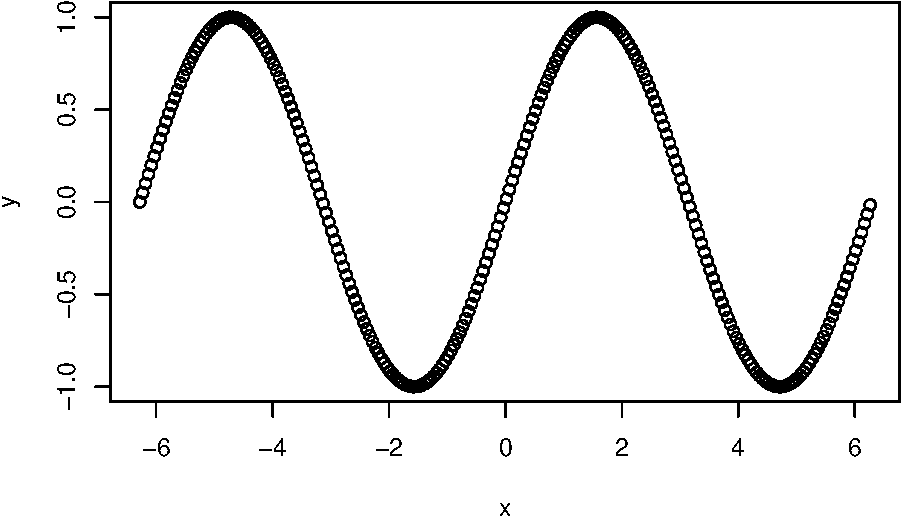
\includegraphics{TUTO_VISU_files/figure-latex/unnamed-chunk-4-1.pdf}

\begin{Shaded}
\begin{Highlighting}[]
\KeywordTok{plot}\NormalTok{(x,y,}\DataTypeTok{type=}\StringTok{"l"}\NormalTok{) }\CommentTok{#représentation sous forme de ligne}
\end{Highlighting}
\end{Shaded}

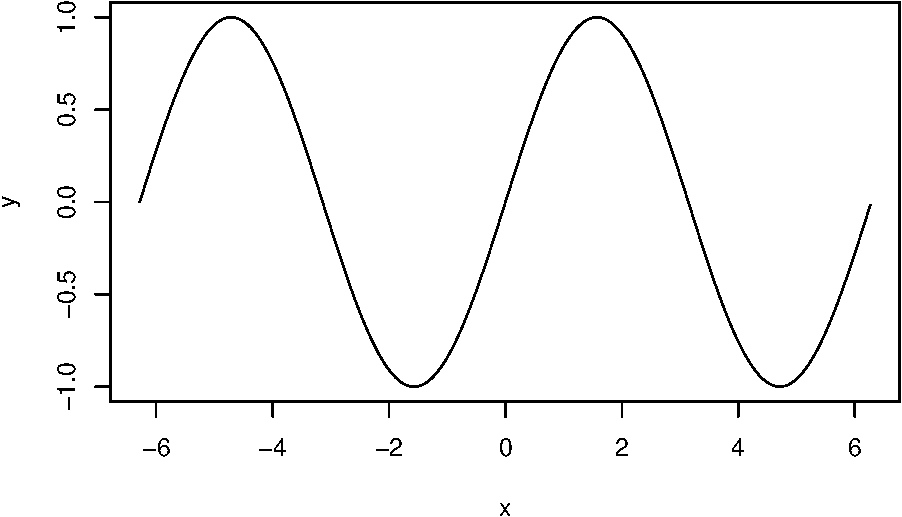
\includegraphics{TUTO_VISU_files/figure-latex/unnamed-chunk-4-2.pdf}

Nous proposons des exemples de représentations de variables quantitatives et qualitatives à l'aide du jeu de données \textbf{ozone.txt} que l'on importe avec

\begin{Shaded}
\begin{Highlighting}[]
\NormalTok{ozone <-}\StringTok{ }\KeywordTok{read.table}\NormalTok{(}\StringTok{"ozone.txt"}\NormalTok{)}
\KeywordTok{summary}\NormalTok{(ozone)}
\end{Highlighting}
\end{Shaded}

\begin{verbatim}
##      maxO3              T9             T12             T15       
##  Min.   : 42.00   Min.   :11.30   Min.   :14.00   Min.   :14.90  
##  1st Qu.: 70.75   1st Qu.:16.20   1st Qu.:18.60   1st Qu.:19.27  
##  Median : 81.50   Median :17.80   Median :20.55   Median :22.05  
##  Mean   : 90.30   Mean   :18.36   Mean   :21.53   Mean   :22.63  
##  3rd Qu.:106.00   3rd Qu.:19.93   3rd Qu.:23.55   3rd Qu.:25.40  
##  Max.   :166.00   Max.   :27.00   Max.   :33.50   Max.   :35.50  
##       Ne9             Ne12            Ne15           Vx9         
##  Min.   :0.000   Min.   :0.000   Min.   :0.00   Min.   :-7.8785  
##  1st Qu.:3.000   1st Qu.:4.000   1st Qu.:3.00   1st Qu.:-3.2765  
##  Median :6.000   Median :5.000   Median :5.00   Median :-0.8660  
##  Mean   :4.929   Mean   :5.018   Mean   :4.83   Mean   :-1.2143  
##  3rd Qu.:7.000   3rd Qu.:7.000   3rd Qu.:7.00   3rd Qu.: 0.6946  
##  Max.   :8.000   Max.   :8.000   Max.   :8.00   Max.   : 5.1962  
##       Vx12             Vx15            maxO3v          vent      pluie   
##  Min.   :-7.878   Min.   :-9.000   Min.   : 42.00   Est  :10   Pluie:43  
##  1st Qu.:-3.565   1st Qu.:-3.939   1st Qu.: 71.00   Nord :31   Sec  :69  
##  Median :-1.879   Median :-1.550   Median : 82.50   Ouest:50             
##  Mean   :-1.611   Mean   :-1.691   Mean   : 90.57   Sud  :21             
##  3rd Qu.: 0.000   3rd Qu.: 0.000   3rd Qu.:106.00                        
##  Max.   : 6.578   Max.   : 5.000   Max.   :166.00
\end{verbatim}

On visualise tout d'abord 2 variables quantitatives à l'aide d'un nuage de points : la concentration en ozone maximale \textbf{maxO3} en fonction de la température à 12h \textbf{T12}.

\begin{Shaded}
\begin{Highlighting}[]
\KeywordTok{plot}\NormalTok{(ozone[,}\StringTok{"T12"}\NormalTok{],ozone[,}\StringTok{"maxO3"}\NormalTok{])}
\end{Highlighting}
\end{Shaded}

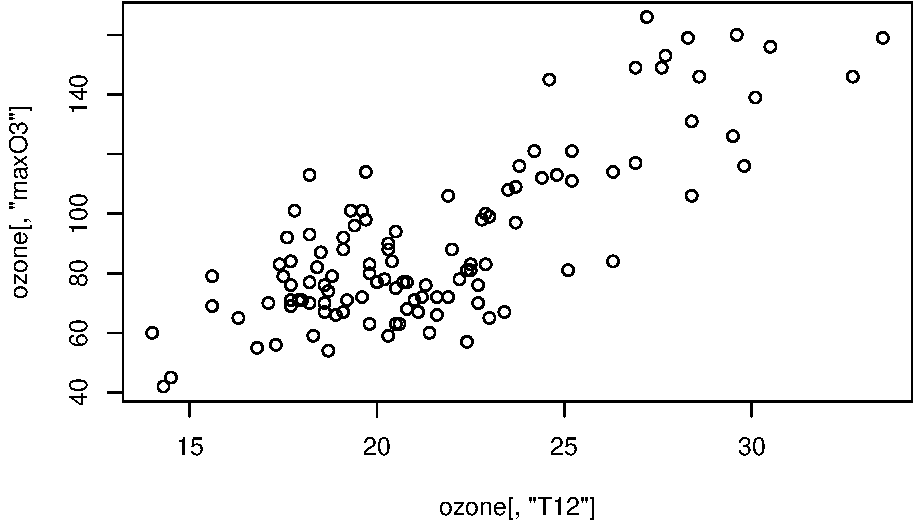
\includegraphics{TUTO_VISU_files/figure-latex/unnamed-chunk-6-1.pdf}

Comme les deux variables appartiennent au même jeu de données, on peut obtenir la même représentation à l'aide d'une sytaxe plus claire qui ajoutent automatiquement les noms des variables sur les axes :

\begin{Shaded}
\begin{Highlighting}[]
\KeywordTok{plot}\NormalTok{(maxO3}\OperatorTok{~}\NormalTok{T12,}\DataTypeTok{data=}\NormalTok{ozone)}
\end{Highlighting}
\end{Shaded}

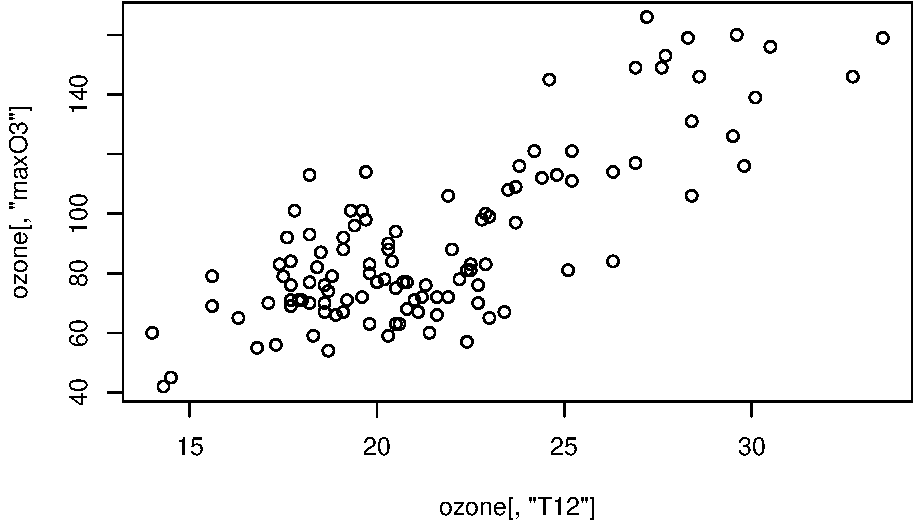
\includegraphics{TUTO_VISU_files/figure-latex/unnamed-chunk-7-1.pdf}

Une autre façon de faire (moins naturelle) :

\begin{Shaded}
\begin{Highlighting}[]
\KeywordTok{plot}\NormalTok{(ozone[,}\StringTok{"T12"}\NormalTok{],ozone[,}\StringTok{"maxO3"}\NormalTok{],}\DataTypeTok{xlab=}\StringTok{"T12"}\NormalTok{,}\DataTypeTok{ylab=}\StringTok{"maxO3"}\NormalTok{)}
\end{Highlighting}
\end{Shaded}

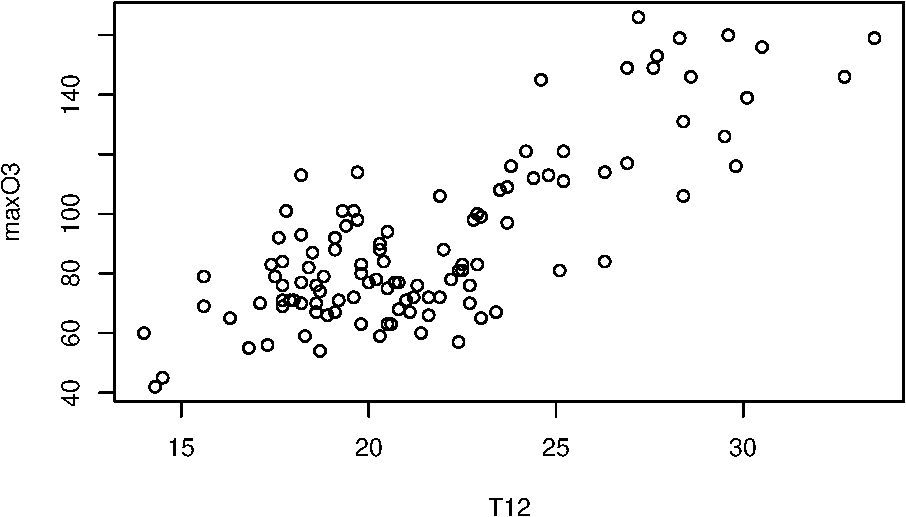
\includegraphics{TUTO_VISU_files/figure-latex/unnamed-chunk-8-1.pdf}

Il existe des fonctions spécifiques pour chaque type de graphs, par exemple \textbf{histogram}, \textbf{barplot} et \textbf{boxplot} :

\begin{Shaded}
\begin{Highlighting}[]
\KeywordTok{hist}\NormalTok{(ozone}\OperatorTok{$}\NormalTok{maxO3,}\DataTypeTok{main=}\StringTok{"Histogram"}\NormalTok{)}
\end{Highlighting}
\end{Shaded}

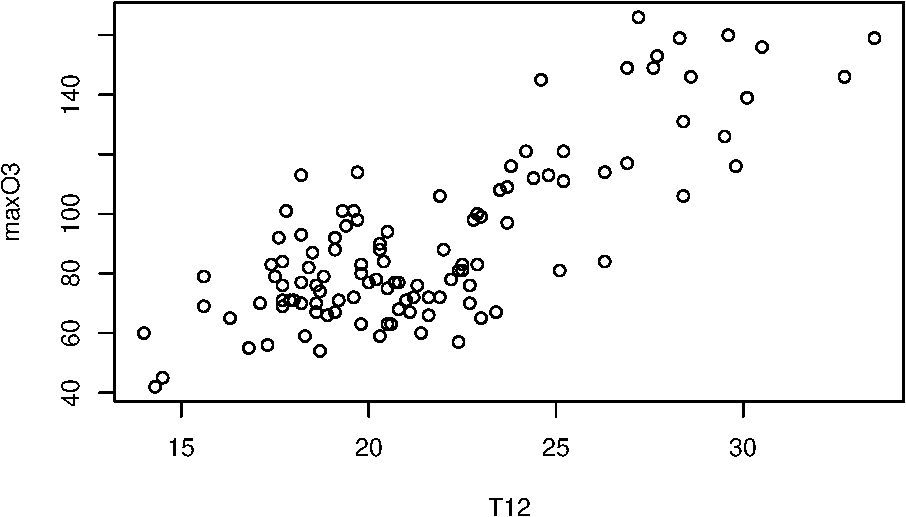
\includegraphics{TUTO_VISU_files/figure-latex/unnamed-chunk-9-1.pdf}

\begin{Shaded}
\begin{Highlighting}[]
\KeywordTok{barplot}\NormalTok{(}\KeywordTok{table}\NormalTok{(ozone}\OperatorTok{$}\NormalTok{vent)}\OperatorTok{/}\KeywordTok{nrow}\NormalTok{(ozone),}\DataTypeTok{col=}\StringTok{"blue"}\NormalTok{)}
\end{Highlighting}
\end{Shaded}

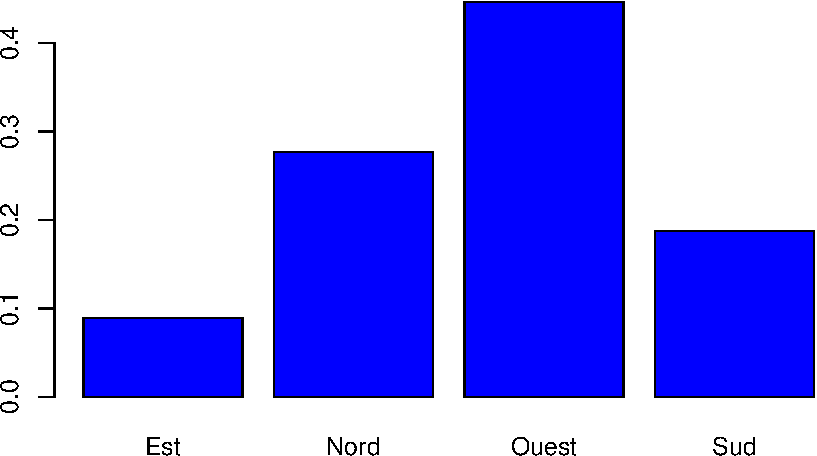
\includegraphics{TUTO_VISU_files/figure-latex/unnamed-chunk-9-2.pdf}

\begin{Shaded}
\begin{Highlighting}[]
\KeywordTok{boxplot}\NormalTok{(maxO3}\OperatorTok{~}\NormalTok{vent,}\DataTypeTok{data=}\NormalTok{ozone)}
\end{Highlighting}
\end{Shaded}

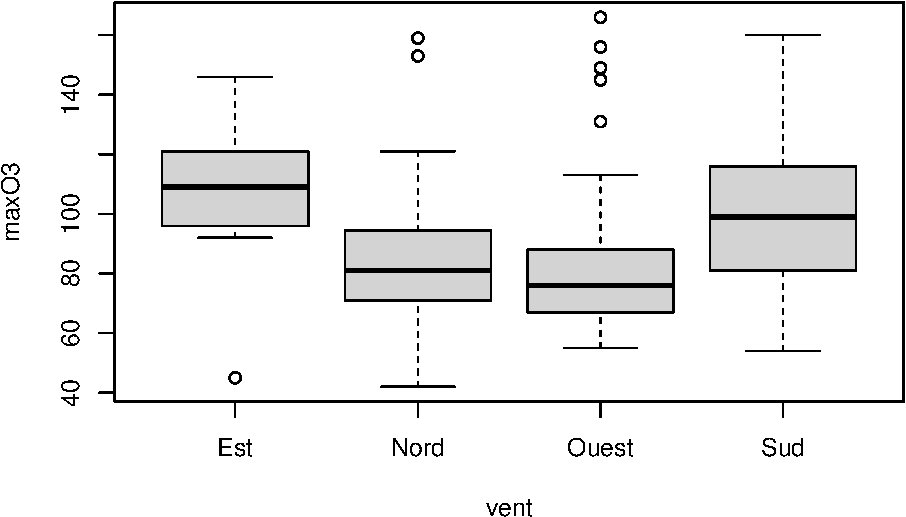
\includegraphics{TUTO_VISU_files/figure-latex/unnamed-chunk-9-3.pdf}

\hypertarget{graphes-interactifs-avec-ramcharts}{%
\subsection{Graphes interactifs avec rAmCharts}\label{graphes-interactifs-avec-ramcharts}}

On peut utiliser ce package pour obtenir des graphes dynamiques. L'utilisation est relativement simple, il suffit d'ajouter le prefixe \textbf{am} devant le nom de la fonction :

\begin{Shaded}
\begin{Highlighting}[]
\KeywordTok{library}\NormalTok{(rAmCharts)}
\KeywordTok{amHist}\NormalTok{(ozone}\OperatorTok{$}\NormalTok{maxO3)}
\end{Highlighting}
\end{Shaded}

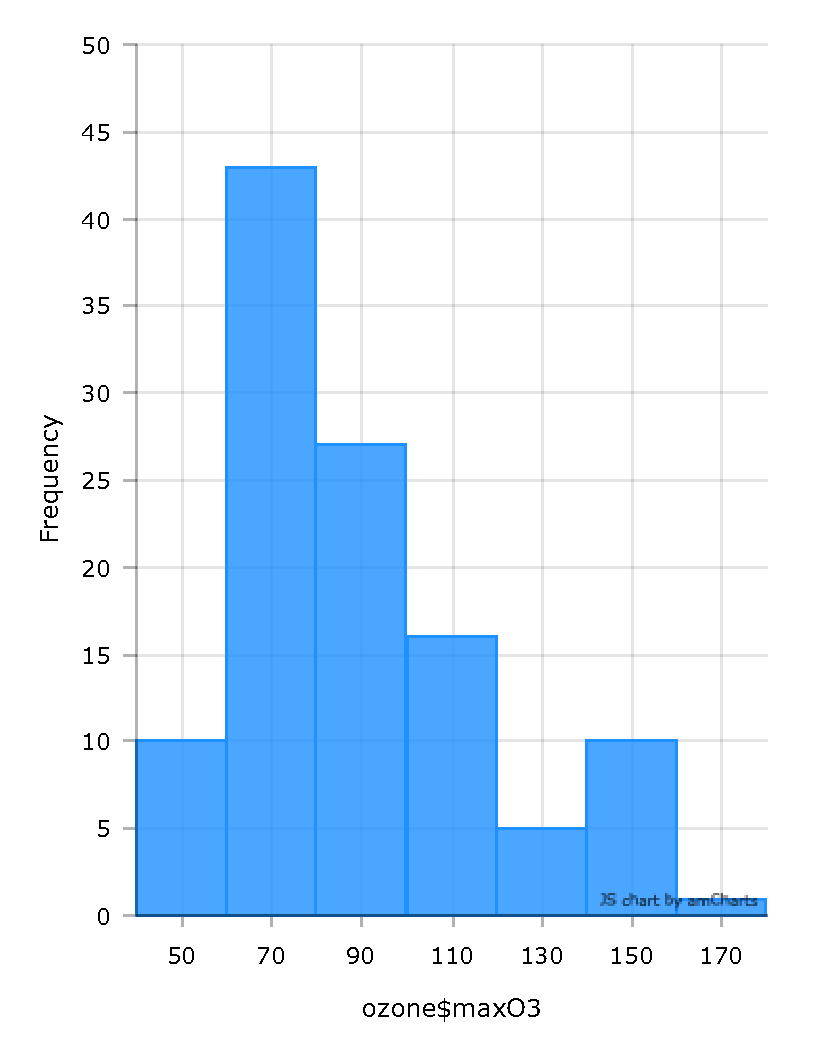
\includegraphics{TUTO_VISU_files/figure-latex/unnamed-chunk-10-1.pdf}

\begin{Shaded}
\begin{Highlighting}[]
\KeywordTok{amPlot}\NormalTok{(ozone,}\DataTypeTok{col=}\KeywordTok{c}\NormalTok{(}\StringTok{"T9"}\NormalTok{,}\StringTok{"T12"}\NormalTok{))}
\end{Highlighting}
\end{Shaded}

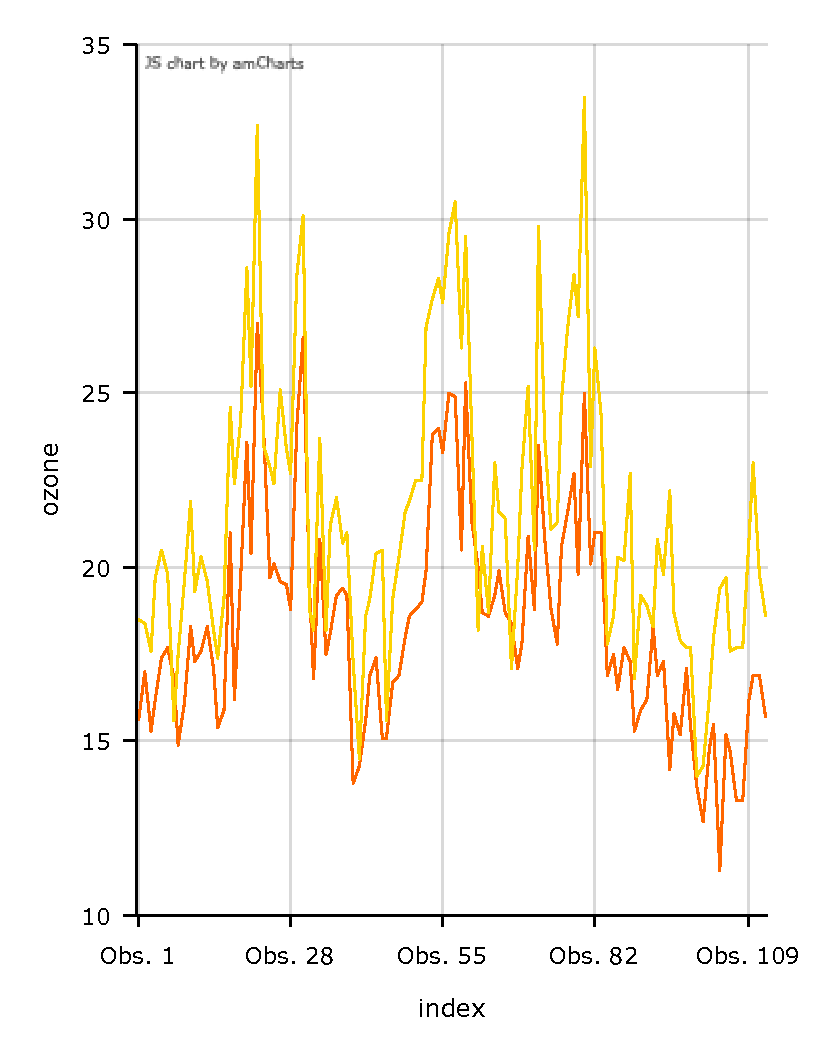
\includegraphics{TUTO_VISU_files/figure-latex/unnamed-chunk-10-2.pdf}

\begin{Shaded}
\begin{Highlighting}[]
\KeywordTok{amBoxplot}\NormalTok{(maxO3}\OperatorTok{~}\NormalTok{vent,}\DataTypeTok{data=}\NormalTok{ozone)}
\end{Highlighting}
\end{Shaded}

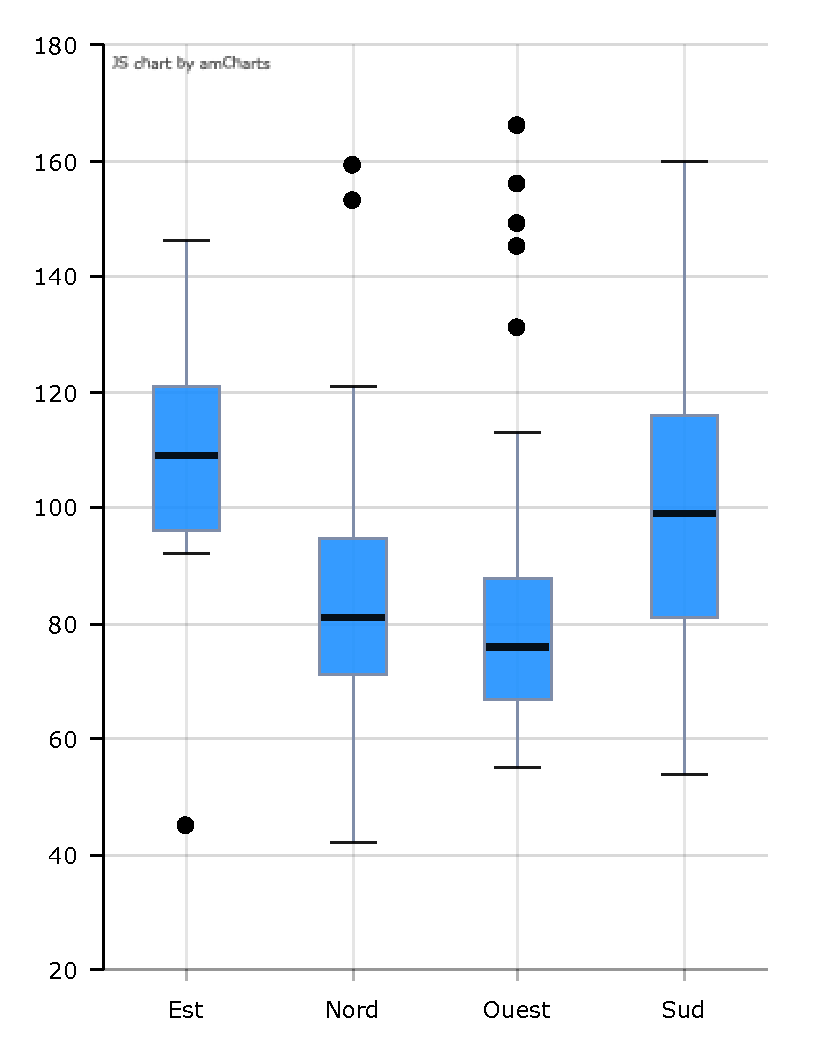
\includegraphics{TUTO_VISU_files/figure-latex/unnamed-chunk-10-3.pdf}

\hypertarget{exercice-1}{%
\subsection{Exercice 1}\label{exercice-1}}

\BeginKnitrBlock{exercise}[Pythagorean theorem]
\protect\hypertarget{exr:exo1}{}{\label{exr:exo1} \iffalse (Pythagorean theorem) \fi{} }

\begin{enumerate}
\def\labelenumi{\arabic{enumi}.}
\tightlist
\item
  Tracer la fonction \textbf{sinus} entre \(0\) et \(2\pi\).
\item
  A l''aide de la fonction \textbf{title} ajouter le titre \textbf{Représentation de la fonction sinus}.

  \EndKnitrBlock{exercise}
\end{enumerate}

\begin{Shaded}
\begin{Highlighting}[]
\NormalTok{x <-}\StringTok{ }\KeywordTok{seq}\NormalTok{(}\DecValTok{0}\NormalTok{,}\DecValTok{2}\OperatorTok{*}\NormalTok{pi,}\DataTypeTok{length=}\DecValTok{1000}\NormalTok{)}
\KeywordTok{plot}\NormalTok{(x,}\KeywordTok{sin}\NormalTok{(x),}\DataTypeTok{type=}\StringTok{"l"}\NormalTok{)}

\KeywordTok{title}\NormalTok{(}\StringTok{"Représentation de la fonction sinus"}\NormalTok{)}
\end{Highlighting}
\end{Shaded}

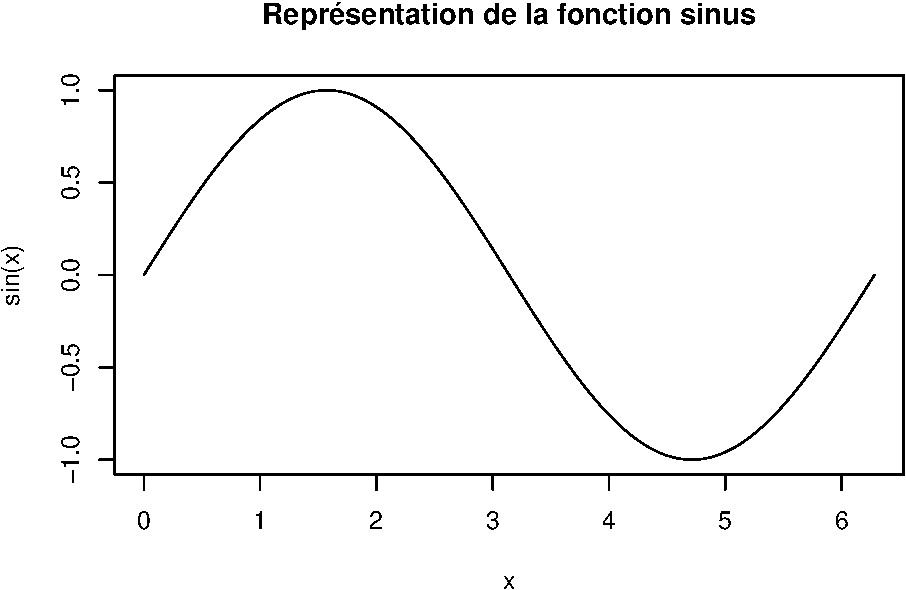
\includegraphics{TUTO_VISU_files/figure-latex/test-a-1.pdf}

\begin{Shaded}
\begin{Highlighting}[]
\CommentTok{# Change the filter to select February rather than January}
\NormalTok{x <-}\StringTok{ }\KeywordTok{seq}\NormalTok{(}\DecValTok{0}\NormalTok{,}\DecValTok{2}\OperatorTok{*}\NormalTok{pi,}\DataTypeTok{length=}\DecValTok{1000}\NormalTok{)}
\KeywordTok{plot}\NormalTok{(x,}\KeywordTok{sin}\NormalTok{(x),}\DataTypeTok{type=}\StringTok{"l"}\NormalTok{)}
\end{Highlighting}
\end{Shaded}

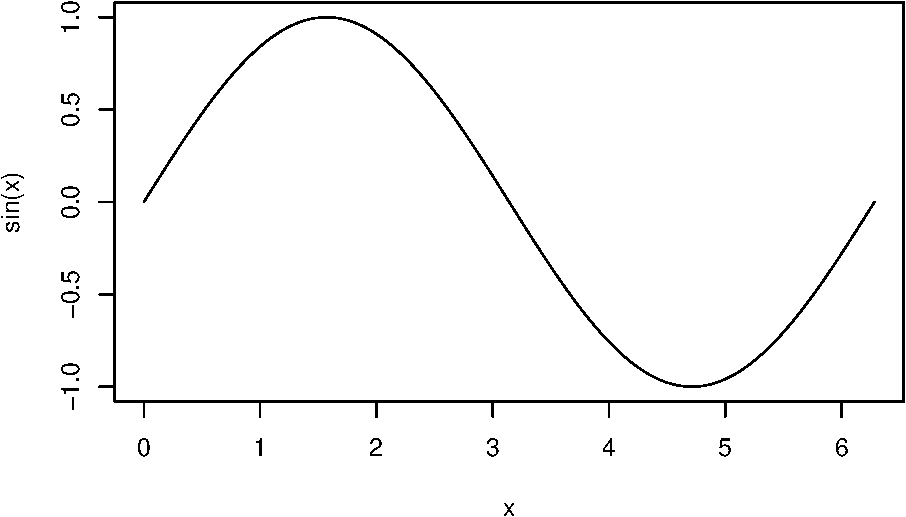
\includegraphics{TUTO_VISU_files/figure-latex/exo2-1.pdf}

\begin{Shaded}
\begin{Highlighting}[]
\NormalTok{x <-}\StringTok{ }\KeywordTok{seq}\NormalTok{(}\DecValTok{0}\NormalTok{,}\DecValTok{2}\OperatorTok{*}\NormalTok{pi,}\DataTypeTok{length=}\DecValTok{1000}\NormalTok{)}
\KeywordTok{plot}\NormalTok{(x,}\KeywordTok{sin}\NormalTok{(x),}\DataTypeTok{type=}\StringTok{"l"}\NormalTok{)}
\end{Highlighting}
\end{Shaded}

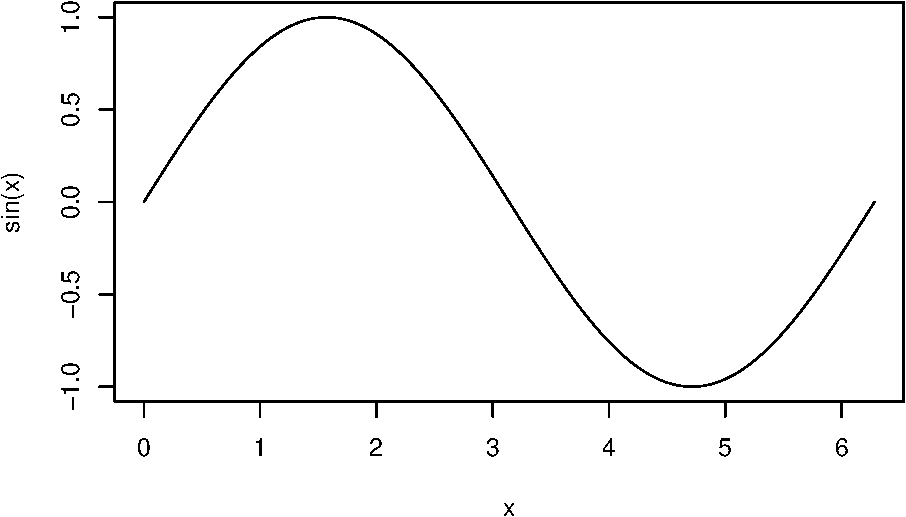
\includegraphics{TUTO_VISU_files/figure-latex/exo2-solution-1.pdf}

\hypertarget{exercice-2}{%
\subsection{Exercice 2}\label{exercice-2}}

\begin{itemize}
\tightlist
\item
  Tracer la densité de la loi normale centrée réduite entre \(-4\) et 4 (utiliser \textbf{dnorm}).
\item
  Ajouter une ligne verticale (en tirets) qui passe par \(x=0\) (utiliser \textbf{abline} avec \textbf{lty=2}).
\item
  Sur le même graphe, ajouter les densités de loi la de Student à 5 et 30 degrés de liberté (utiliser \textbf{dt}). On utilisera la fonction \textbf{lines} et des couleurs différentes pour chaque densité.
\item
  Ajouter une légende qui permet de repérer chaque densité (fonction \textbf{legend}).
\end{itemize}

\begin{Shaded}
\begin{Highlighting}[]
\NormalTok{x <-}\StringTok{ }\KeywordTok{seq}\NormalTok{(}\OperatorTok{-}\DecValTok{4}\NormalTok{,}\DecValTok{4}\NormalTok{,}\DataTypeTok{by=}\FloatTok{0.01}\NormalTok{)}
\KeywordTok{plot}\NormalTok{(x,}\KeywordTok{dnorm}\NormalTok{(x),}\DataTypeTok{type=}\StringTok{"l"}\NormalTok{)}
\KeywordTok{abline}\NormalTok{(}\DataTypeTok{v=}\DecValTok{0}\NormalTok{,}\DataTypeTok{lty=}\DecValTok{2}\NormalTok{)}

\KeywordTok{lines}\NormalTok{(x,}\KeywordTok{dt}\NormalTok{(x,}\DecValTok{5}\NormalTok{),}\DataTypeTok{col=}\DecValTok{2}\NormalTok{)}
\KeywordTok{lines}\NormalTok{(x,}\KeywordTok{dt}\NormalTok{(x,}\DecValTok{30}\NormalTok{),}\DataTypeTok{col=}\DecValTok{3}\NormalTok{)}

\KeywordTok{legend}\NormalTok{(}\StringTok{"topleft"}\NormalTok{,}\DataTypeTok{legend=}\KeywordTok{c}\NormalTok{(}\StringTok{"normal"}\NormalTok{,}\StringTok{"Student(5)"}\NormalTok{,}\StringTok{"Student(30)"}\NormalTok{),}\DataTypeTok{col=}\DecValTok{1}\OperatorTok{:}\DecValTok{3}\NormalTok{,}\DataTypeTok{lty=}\DecValTok{1}\NormalTok{)}
\end{Highlighting}
\end{Shaded}

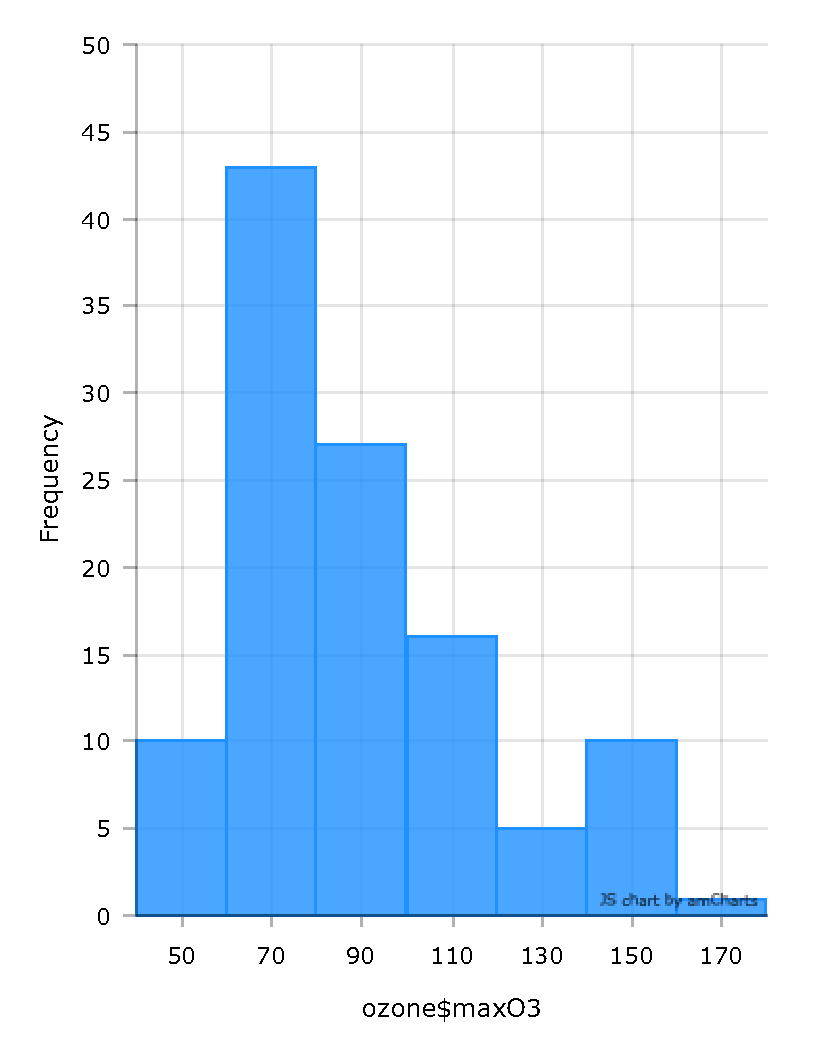
\includegraphics{TUTO_VISU_files/figure-latex/unnamed-chunk-11-1.pdf}

You can label chapter and section titles using \texttt{\{\#label\}} after them, e.g., we can reference Chapter \ref{intro}. If you do not manually label them, there will be automatic labels anyway, e.g., Chapter \ref{methods}.

Figures and tables with captions will be placed in \texttt{figure} and \texttt{table} environments, respectively.

\begin{Shaded}
\begin{Highlighting}[]
\KeywordTok{par}\NormalTok{(}\DataTypeTok{mar =} \KeywordTok{c}\NormalTok{(}\DecValTok{4}\NormalTok{, }\DecValTok{4}\NormalTok{, }\FloatTok{.1}\NormalTok{, }\FloatTok{.1}\NormalTok{))}
\KeywordTok{plot}\NormalTok{(pressure, }\DataTypeTok{type =} \StringTok{'b'}\NormalTok{, }\DataTypeTok{pch =} \DecValTok{19}\NormalTok{)}
\end{Highlighting}
\end{Shaded}

\begin{figure}

{\centering 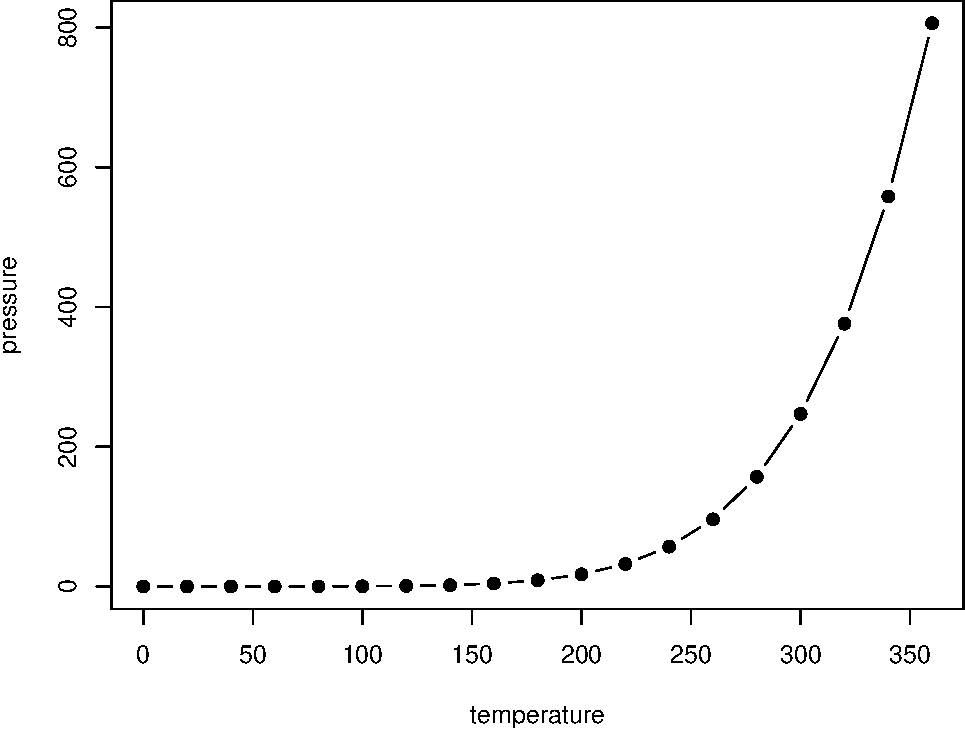
\includegraphics[width=0.8\linewidth]{TUTO_VISU_files/figure-latex/nice-fig-1} 

}

\caption{Here is a nice figure!}\label{fig:nice-fig}
\end{figure}

Reference a figure by its code chunk label with the \texttt{fig:} prefix, e.g., see Figure \ref{fig:nice-fig}. Similarly, you can reference tables generated from \texttt{knitr::kable()}, e.g., see Table \ref{tab:nice-tab}.

\begin{Shaded}
\begin{Highlighting}[]
\NormalTok{knitr}\OperatorTok{::}\KeywordTok{kable}\NormalTok{(}
  \KeywordTok{head}\NormalTok{(iris, }\DecValTok{20}\NormalTok{), }\DataTypeTok{caption =} \StringTok{'Here is a nice table!'}\NormalTok{,}
  \DataTypeTok{booktabs =} \OtherTok{TRUE}
\NormalTok{)}
\end{Highlighting}
\end{Shaded}

\begin{table}

\caption{\label{tab:nice-tab}Here is a nice table!}
\centering
\begin{tabular}[t]{rrrrl}
\toprule
Sepal.Length & Sepal.Width & Petal.Length & Petal.Width & Species\\
\midrule
5.1 & 3.5 & 1.4 & 0.2 & setosa\\
4.9 & 3.0 & 1.4 & 0.2 & setosa\\
4.7 & 3.2 & 1.3 & 0.2 & setosa\\
4.6 & 3.1 & 1.5 & 0.2 & setosa\\
5.0 & 3.6 & 1.4 & 0.2 & setosa\\
\addlinespace
5.4 & 3.9 & 1.7 & 0.4 & setosa\\
4.6 & 3.4 & 1.4 & 0.3 & setosa\\
5.0 & 3.4 & 1.5 & 0.2 & setosa\\
4.4 & 2.9 & 1.4 & 0.2 & setosa\\
4.9 & 3.1 & 1.5 & 0.1 & setosa\\
\addlinespace
5.4 & 3.7 & 1.5 & 0.2 & setosa\\
4.8 & 3.4 & 1.6 & 0.2 & setosa\\
4.8 & 3.0 & 1.4 & 0.1 & setosa\\
4.3 & 3.0 & 1.1 & 0.1 & setosa\\
5.8 & 4.0 & 1.2 & 0.2 & setosa\\
\addlinespace
5.7 & 4.4 & 1.5 & 0.4 & setosa\\
5.4 & 3.9 & 1.3 & 0.4 & setosa\\
5.1 & 3.5 & 1.4 & 0.3 & setosa\\
5.7 & 3.8 & 1.7 & 0.3 & setosa\\
5.1 & 3.8 & 1.5 & 0.3 & setosa\\
\bottomrule
\end{tabular}
\end{table}

You can write citations, too. For example, we are using the \textbf{bookdown} package \citep{R-bookdown} in this sample book, which was built on top of R Markdown and \textbf{knitr} \citep{xie2015}.

\hypertarget{literature}{%
\chapter{Literature}\label{literature}}

Here is a review of existing methods.

\hypertarget{methods}{%
\chapter{Methods}\label{methods}}

We describe our methods in this chapter.

\hypertarget{applications}{%
\chapter{Applications}\label{applications}}

Some \emph{significant} applications are demonstrated in this chapter.

\hypertarget{example-one}{%
\section{Example one}\label{example-one}}

\hypertarget{example-two}{%
\section{Example two}\label{example-two}}

\hypertarget{final-words}{%
\chapter{Final Words}\label{final-words}}

We have finished a nice book.

\bibliography{book.bib,packages.bib}

\end{document}
